\begin{frame}
\frametitle{PIB Colombia \small{(Elaboración propia con base en DANE)}}
\begin{center}
\resizebox{\textwidth}{!}{
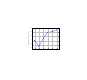
\begin{tikzpicture}[scale=0.04]
\begin{axis}[
    width=10cm,
    height=8cm,
    ylabel={PIB (Normalizado a 2019=1)},
    xtick={0, 1, 2, 3, 4, 5},
    xticklabels={2019, 2020, 2021, 2022, 2023, 2024},
    x tick label style={rotate=90, anchor=east},
    ymin=0.9,
    ymax=1.15, % Adjusted ymax for better fit
    grid=both,
    grid style=dashed,
    thick
]
% PIB Normalizado
\addplot[color=blue, mark=*, solid] coordinates {
    (0,1.00) 
    (1,0.9281) 
    (2,1.0284)
    (3, 1.1033)
    (4, 1.1101)
    (5, 1.1312) 
};
\end{axis}
\end{tikzpicture}
%\vspace{0.3cm}
%\par\footnotesize{\textit{Fuente: Cálculos propios con base en el DANE}}
%\end{figure}
}
\end{center}
\end{frame}
